\chapter{Starting the GUI}
\label{s:gui.startup}

From your system shell, you can execute the gui with the command
\begin{example}
  python -m pytao.gui
\end{example}
You can also specify any of the command line options that tao supports.  For example,
\begin{example}
  python -m pytao.gui -init_file ~/bmad_dist/tao/examples/cesr/tao.init -rf_on
\end{example}
This will prefill the settings for \texttt{init_file} and \texttt{rf_on}.
The GUI starts with the window shown in Figure \ref{fig:startup}.
From here, all of the command-line settings that Tao supports can be set (settings that are left blank are omitted when Tao is started).

Towards the bottom of the window are some settings that are specific to the GUI.  The "Interface to Tao" setting controls whether the ctypes or pexpect backend for communicating with Tao will be used.
Below it, the "Shared Library" or "Tao executable" setting points the GUI to the correct executable or shared object library to use.
In most cases, the GUI will prefill this box by referencing the ACC_LOCAL_ROOT and ACC_ROOT_DIR environmental variables.

Finally, the font size can be set as desired.
Hitting Enter/Return while the font size box is in focus will adjust the font size of the startup window to give the user a sense of what the chosen font size will look like.

Once all of the startup settings have been set, clicking "Start Tao" will initialize Tao and bring the user to the main GUI window.
\begin{figure}
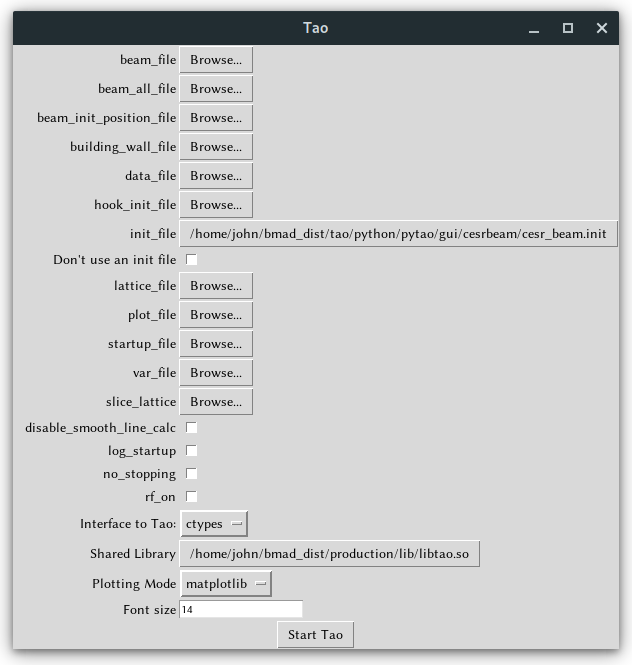
\includegraphics[width=8cm]{figures/startup.png}
\centering
\caption{The GUI startup window.  In this example, the init file that tao should use has been specified.}
\label{fig:startup}
\end{figure}

%--------------------------------------------------------------

\section{GUI Initialization File}
\label{s:gui.init.file}

To speed up the initialization process, you can make an init file for the GUI.  This file should be called "gui.init", and it should be in the same directory from which you initialize the GUI.

gui.init should have each option on a separate line, and each option should be listed in the form "parameter:value".  For example, the text below would constitute a good gui.init file:

\begin{example}
  #MY GUI INIT FILE
  beam_file:/path/to/beam/file
  data_file:/path/to/data/file
  #THIS IS A COMMENT
  disable_smooth_line_calc:T
  rf_on:T
  tao_exe:/path/to/executable
\end{example}

The order in which you list options in gui.init is not important.

File paths should be specified in full to be safe, but you can specify paths relative to the directory from which you launch main.py.  For example, "/home/username/file", "subfolder/my_file", and "../../path/to/another/file" would all be acceptable file paths.  You can also use your environmental variables and "\textasciitilde{}", as in "\textasciitilde{}/Documents/my_file" and "\$DIST_BASE_DIR/tao/file".

Logic (true/false) options may be specified by T/F or True/False.

You can also include comments with \#.  Anything after a \# character will be ignored.

To get a list of parameters that can be set in a \vn{gui.init} file, start Tao with the command
\begin{example}
  tao -help
\end{example}
The corresponding gui.init parameter is the Tao parameter with the leading dash "-" removed and a
colon ":" between the parameter and the parameter's value. For logical parameters, for example,
"rf_on", Use T/F or True/False as the parameter's value.

